% ============================================================
% f2014_beijing_science_q15_triangle.tex
% 2014 北京卷（理科）第 15 题：三角形 ABC 与点 D
% 来源 PDF：普通高考/2014/2014北京理.pdf
% 原页：第 1 页（A3），印面 861，中栏第 15 题题干下方
% 已知 ∠B=π/3，AB=8，CD=2；图按 AB=8、BD=3、DC=2、AC=7 的真实比例绘制。
% ============================================================
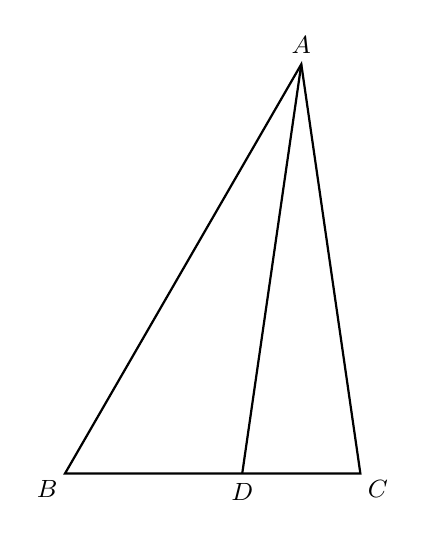
\begin{tikzpicture}[scale=0.75, line width=0.8pt, font=\small]
  \coordinate (B) at (0,0);
  \coordinate (D) at (3,0);
  \coordinate (C) at (5,0);
  \coordinate (A) at (4,6.9282);   % AB=8，∠B=60°

  \draw (A) -- (B) -- (C) -- cycle;
  \draw (A) -- (D);

  \node[above] at (A) {$A$};
  \node[below left=-1pt] at (B) {$B$};
  \node[below] at (D) {$D$};
  \node[below right=-1pt] at (C) {$C$};
\end{tikzpicture}
